\documentclass{article}
\usepackage{CJKutf8}
\usepackage{multicol}
% Packages
\usepackage{lipsum} % For generating dummy text
\usepackage[top=1in, bottom=1in, left=1in, right=1in]{geometry}
\usepackage{hyperref}
\usepackage{pgfplots}
\usetikzlibrary{pgfplots.polar}
\usepackage{caption}
\captionsetup{font=small}
\usepackage{standalone}
\usepackage{listings}
\usepackage{xcolor} % For setting colors
\usepackage{amssymb}
\usepackage{amsmath}
\usepackage{algorithm}
\usepackage{algpseudocode}
\usepackage{afterpage}
\usepackage{placeins}
\usepackage{tikz}
\usepackage{enumitem}
\lstset{
  language=TeX,
  breaklines=true,
  basicstyle=\ttfamily\small,
  keywordstyle=\color{blue},
  commentstyle=\color{green},
  backgroundcolor=\color{gray!10},
  frame=single,
  showspaces=false,
  showstringspaces=false,
}
\pgfplotsset{compat=1.17} % Use this to ensure compatibility with newer features
\setlength{\parskip}{6pt}
% Title and author

\title{Autonomous Competence Identification Protocol: A Dynamic Ranking Ladder System for Blockchain Applications}

\author{Tim Pechersky, Aivars Smirnovs}

\begin{document}
\begin{CJK}{UTF8}{gbsn}

    % \twocolumn
    \maketitle

    \begin{abstract}
        This paper introduces the Autonomous Competence Identification Protocol (ACIP), a novel dynamic ranking ladder system for trustless environments. ACIP leverages game-theoretic principles and dynamic systems theory to autonomously identify and reward competence while mitigating Sybil attacks. Participants compete in time-locked, tiered groups, progressing through ranks based on peer-validated competence. This protocol establishes a quantifiable, verifiable, and potentially tokenized measure of competence—which can be conceptualized as a multi-dimensional vector representing diverse skills and expertise—secured by participants' commitment of time and financial resources, and culminates in a system of peer-recognized governance over collective reward treasuries, which can further empower recognized competence by serving as backing for attested rank tokens. ACIP offers a robust foundation for merit-based blockchain consensus, decentralized governance, and equitable online communities, moving beyond purely power-based systems.
    \end{abstract}

    \section{Introduction}

    Traditional meritocratic models struggle to objectively identify and reward competence.\cite{Arrow2000} This challenge is significantly amplified in decentralized systems, where trust is minimized and the risk of manipulation is high.  \cite{Rainer2023}\cite{Robin22}\cite{Xuan2024}

    This paper introduces a novel protocol to establish a dynamic ranking ladder system. Our protocol incentivizes participants to demonstrate their abilities through competitive "elections" within tiered groups. By requiring time and financial commitment, we create a system resistant to Sybil attacks and foster genuine competence development. ACIP moves beyond a monolithic score, allowing for the representation and validation of competence across multiple dimensions, where the same foundational asset commitment (time and resources) can contribute to distinct expertise vectors. Group entry can be predicated on specific combinations of these dimensional competences, fostering a rich "multiverse" of specialized domains whose interrelations can be analyzed (e.g., via cosine similarity between competence vectors). This approach can be applied to various decentralized systems, including blockchain consensus mechanisms, offering not only a measure of individual competence but also a framework for collective reward governance by high-ranking peers, whereby collective treasuries can be utilized by recognized competence organizations or \textit{guilds} to stake against and validate the rank tokens of their endorsed members, effectively creating a backed Proof of Competence. contributing to more robust and equitable governance.

    Empirically, the protocol's dynamics can be observed in many online games. In these games, participants engage in competitions, and winners emerge through a process that inherently validates the protocol's core principles.

        {{Furthermore, the structured interactions and peer-validation processes within ACIP, especially when combined with protocols like CVPP \cite{cvpp} for content generation, offer a novel pathway to create high-quality, domain-specific datasets. These datasets, inherently ranked and categorized by competence dimensions, can be directly utilized for training and evaluating Machine Learning models, providing a significant advantage over less structured or unverified data sources.}}

    This research aims to:

    \begin{itemize}[nosep]
        \item Propose a methodology for creating a dynamic ranking system in a trustless environment.
        \item Analyze attack vectors and present robust resistance mechanisms.
        \item Discuss applications and benefits of the competence framework.
    \end{itemize}

    The proposed protocol is a theoretical construct that relies on established consensus mechanisms to operate. It can be executed on existing blockchain protocols.

    \section{Protocol Overview}

    The Autonomous Competence Identification Protocol (ACIP) establishes a dynamic ranking ladder through a series of tiered groups and competitive interactions. Participants progress through ranks by demonstrating competence within these groups. The core components of the protocol are time-based participation and cost-based commitment, ensuring robustness and Sybil resistance.

    The protocol operates through the following steps:

    \begin{enumerate}
        \item \textbf{Group Formation:} Participants join groups based on shared interests or topics. Groups are tiered, representing different levels of competence and may define entry requirements based on specific profiles of dimensional competence.
        \item \textbf{Time-Locked Participation:}  Participation in a group requires a time commitment ($T_{id}$), ensuring sustained engagement.
        \item \textbf{Cost-Based Commitment:} Joining a group and progressing in rank requires a financial stake ($X_{id}$), deterring Sybil attacks and frivolous participation.
        \item \textbf{Competitive Interaction ("Elections"):} Within each group, participants engage in a competitive process (e.g., voting, proposal evaluation, debate) to identify the most competent individuals along one or more defined dimensions of competence.
        \item \textbf{Rank Advancement:} Winners of the competitive process within a group advance to higher ranks within the relevant competence dimension(s), reflecting their demonstrated competence. Losers remain in their current rank or may descend based on protocol rules.
        \item \textbf{Dynamic Rank Adjustment:} Ranks (or dimensional competence scores) are not static; they are dynamically adjusted based on ongoing participation and performance in group competitions.
        \item \textbf{Competence Representation:}  Rank $R$ is generalized to a competence vector $\vec{P_c} = (c_1, c_2, ..., c_n)$, where each component represents proficiency in a distinct dimension. This vector is represented and stored on-chain, providing a verifiable and transparent measure of multi-dimensional competence. This can be tokenized or used as a reputation profile within the decentralized system.
        \item \textbf{Advanced Peer Recognition \& Treasury Governance:} At higher ranks, sustained competence can be further validated by the collective of established high-rank peers. This may grant governance rights over communal reward treasuries (funded by participation costs) and the ability to claim value from them. Furthermore, recognized high-rank organizations or \textit{guilds} may leverage these treasury assets to "bake" or stake against the rank tokens or specific dimensional competence scores of individuals they endorse, thereby creating a more robust, value-backed Proof of Competence.
    \end{enumerate}

    This dynamic process creates a self-regulating ranking ladder where competence is continuously assessed and rewarded. The time and cost components ensure that rank is not easily gained through manipulation or superficial effort.

    Within the framework of ACIP, we formally define competence as: the measure of time and financial resources an individual is willing to commit to a specific domain, validated by the peer-assessed recognition of this commitment and resulting skill or insight they receive from fellow participants within that domain. This initial peer validation occurs through the group's election process. The ultimate validation of profound and sustained competence, however, may come from a further layer of recognition by the collective of established high-rank peers. This higher-order peer acceptance is crucial for an individual to gain significant governance influence over, or access to, shared resources such as the communal Rewards Treasury, signifying their trustworthiness and acknowledged leadership within the ecosystem. Moreover, such established competence can be further amplified when recognized \textit{guilds} or organizations, themselves composed of high-rank peers, choose to stake portions of the collective Rewards Treasury to "bake" or financially back the rank tokens of individuals they endorse, transforming their rank into a directly collateralized Proof of Competence.

    \section{Detailed Protocol Specifications}

    The protocol breaks participants into smaller groups to elect a winner. This election can be implemented as any sub-protocol like a block building challenge, community discussion, or general data exchange, which isn't discussed here. For instance, in a data exchange context, competence could be assessed based on the quality, relevance, or verifiability of the data contributed, with peers voting on the contributions. It involves multiple participants agreeing on a verifiable leader.

    We introduce two principal constant values for our protocol to make groups interoperable based on the same trust assumptions, yet free to define their own participation parameters: (1) principal time constant $P_t$ and (2) principal asset cost $P_c$. These create a common price and time relationship between groups. We also add a boundary case limitation $N_{min}$ - minimum number of participants required to form a group.

    Besides protocol-wide constants, we allow each group to have its own properties:

    \begin{itemize}[nosep]
        \item id - a protocol-wide unique group identifier
        \item $N$ - number of participants
        \item $T$ - minimum time agreed by members to finalize election
        \item $R$ - rank
        \item $S$ - state - can be:
              \begin{itemize}[nosep]
                  \item \textbf{created} - group is created and waiting for participants.
                  \item \textbf{started} - group starts $ts_i$ time of start is recorded
                  \item \textbf{finalized} - group is finalized
              \end{itemize}
              % \item $X$ - stake requirement
    \end{itemize}

    Additionally, there are two global properties for each participant:

    \begin{itemize}[nosep]
        \item  $UID$ - a unique participant identifier
        \item  $\vec{P_r}$ - participant's current competence vector (e.g., $(c_1, c_2, ..., c_n)$)
        \item $P_g$ - group id last joined by participant
    \end{itemize}

    Participants can change groups only if their current and target group are not in "started" state. Whenever someone starts a group, it must have at least $N_{min}$ participants and result in an irreversible total participation commitment or cost $X_{id}$ for the group event, to which all participants contribute their individual share (as defined in Eq. \ref{eq:join-fee}). This commitment, $X_{id}$, while often financial, can more broadly represent any verifiable and committed resource, such as attested platform usage, computational work, or educational credits, as discussed further in Section \ref{sec:utility_and_treasury}.
    \begin{equation}
        \label{eq:group-fee}
        X_{id} = f(T_{id}) = \dfrac{P_t \cdot  P_c }{T_{id}}
    \end{equation}

    These costs can be broken down into equal stakes subtracted from each participant's account whenever group changes its state to "started":
    \begin{equation}
        \label{eq:join-fee}
        stake = \dfrac{X_{id}}{ N_{id}}
    \end{equation}
    The total group participation cost $X_{id}$ can be conceptualized as a sum of distinct components:
    \begin{equation}
        X_{id} = X_{id,reward} + X_{id,data} + X_{id,comp}
    \end{equation}
    Where $X_{id,reward}$ is the component of the participation cost primarily designated to fund the communal Rewards Treasury (as detailed in Section \ref{sec:utility_and_treasury}); a smaller fraction might optionally be allocated for immediate incentives to the direct winner of the group, but the main portion contributes to the collectively governed treasury. $X_{id,data}$ covers data retention costs associated with the group's activities (e.g., storing discussion records, voting history), and $X_{id,comp}$ accounts for computational and network operational expenses. Consequently, each participant's individual stake ($stake = X_{id} / N_{id}$) also implicitly contributes to these components. The precise allocation between these components can be defined by the group or the overarching protocol governance.
    \input{ladder.tex}
    The concept of "irreversible" implies that no participant of group is getting back their stake at full value. This is a key feature of the protocol that ensures the ranking system isn't manipulated by financial power. The stake instead can be channeled for protocol utility operations, data retention in case of storage heavy applications like \cite{cvpp} may be. While the primary stake is irreversible, a portion of collected fees potentially exceeding the baseline cost to secure against Sybil attacks (informed by estimations like Eq. \ref{eq:sybil_cost_one_group_expected}) could be allocated to a reward pool for winners. However, this must be carefully calibrated, as directly rewarding with the full stake significantly lowers collusion resistance and would necessitate additional mechanisms such as proof of humanity \cite{WorldCoin2024} or robust collusion detection, alongside clear advisories to participants regarding these risks.



    The group can finalize only after $T_{i}$ has elapsed since the start state transition and start transition must be recorded on the underlying consensus or similar, guaranteeing the visibility of the start transition for other ranking ladder competitors globally.

    A winner can be declared and their competence vector $\vec{P_r}$ in the state trie updated (e.g., incrementing a specific dimensional component $c_j$ or a composite score) only if the participant meets the group's criteria for advancement, which may involve their existing competence profile $\vec{P_r}$ aligning with the group's rank $R$ or its dimensional focus. This process can repeat and is illustrated in Fig. \ref*{fig:game-connection}.

    \paragraph{Dynamic Proof-of-Authority.} Unlike traditional Proof-of-Authority systems that rely on pre-vetted validators, ACIP introduces a dynamic form where authority (represented by the competence vector $\vec{P_r}$) is earned and continuously validated through participation and peer assessment. Each successful participation in a group instance $id$ incurs a cost $X_{id}$ and results in an update to the participant's competence vector $\vec{P_r}$. The total economic commitment to reach a specific state of the competence vector $\vec{P_r}$ can be seen as the sum of costs $X_{id}$ for all group participations that contributed to achieving that state. For a simplified view, if we consider increments along a primary dimension or an aggregated score, the cumulative cost to reach a level $L$ from $L-1$ can be expressed as:
    \begin{equation}
        \label{eq:time-weighted-proof-of-authority}
        \$_{L} = \$_{L-1} + X_{id, (L-1)}
    \end{equation}
    where $\$_{L}$ is the total cumulative cost to achieve a certain level $L$ of competence (potentially in a specific dimension or as an aggregate score), and $X_{id, (L-1)}$ is the total participation cost for the group successfully completed to transition from level $L-1$ to $L$.

        For analyzing the rate of progression, if an agent repeatedly participates in and wins group instances. For this analysis, let $id$ refer not to a single unique group instance, but rather to a specific *configuration* or *type* of group that the agent consistently chooses. Such a group type is characterized by a fixed election duration, denoted $T_{type}(id)$, and a corresponding participation cost, $X_{type}(id)$ (derived from $T_{type}(id)$ via Eq. \ref{eq:group-fee}). The maximum number of such successful participations, $N_{participations}(t_{total}, id_{type})$, over a total elapsed protocol time $t_{total}$ is:
        \begin{equation}
            \label{eq:max-participations} % Renamed from eq:max-rank-steps
            N_{participations}(t_{total}, id_{type}) = \dfrac{t_{total}}{T_{type}(id_{type})}
        \end{equation}
        It is important to note that if an agent builds their competence vector by participating in a sequence of groups where each group $k$ has a potentially different duration $T(id_k)$, the total time taken would be the sum $\sum T(id_k)$. Equation \ref{eq:max-participations}, however, analyzes repeated engagement with a single group type.

        Substituting into Eq. \ref{eq:max-participations}, we get:
        \begin{equation}
            \label{eq:max-participations-cost} % Renamed from eq:max-rank-steps-cost
            N_{participations}(t_{total}, id_{type}) = \dfrac{t_{total} \cdot X_{type}(id_{type})}{P_t \cdot P_c}
        \end{equation}
        This formulation (Eq. \ref{eq:max-participations-cost}) clearly illustrates the "time-money" relationship: achieving a higher number of successful participations (and thus competence vector updates) within a given $t_{total}$ in a specific type of group necessitates choosing group types with a higher $X_{type}(id_{type})$ (implying shorter $T_{type}(id_{type})$), demanding greater financial commitment per unit of time.

        \paragraph*{Frequency domain.} Eq. \ref{eq:max-participations-cost} highlights the dynamic nature of the protocol. Since it shows linear-time invariant property, the dynamic systems theory \cite{Lynn86} may be applied to analyze its stability and predict its future behavior. $T_{type}(id_{type})$ is a specific minimal time to finalize a group election of group type characterized by $id_{type}$.

    $1/T_{type}(id_{type})$ represents frequency, hence phase and frequency relationships between groups exist. Analysis may be done in s-domain using Laplace transforms.

        Different groups (now understood as group types characterized by $id_{type}$) with different $T_{type}(id_{type})$ would result in a dynamic competence ladder that can allow for the formation of effective ruling coalitions at specific times and due to limited resources to stake and irreversible nature of the stake, even if an effective ruling coalition emerges, its dominance is temporary and accommodates for time division multiplexing between competing groups.

        The emergence and prevalence of group types with specific $T_{type}(id_{type})$ and corresponding $X_{type}(id_{type})$ parameters may also be influenced by external market demands. For instance, if the ranking process within certain group types produces valuable work or data as a byproduct, there might be a greater tolerance or demand for faster (and thus more expensive) ranking cycles within those domains. Conversely, if the primary demand is for highly vetted, top-tier ranking experts, longer and potentially less costly (per cycle) group durations that emphasize thoroughness might be favored. This interplay can lead to a diverse ecosystem of group configurations, each optimizing the time/cost balance based on the specific utility or output valued by its participants and the broader market.

        \subsection{Multi-Dimensional Competence and the Competence Multiverse}
        \label{sec:multi_dimensional_competence}

        ACIP extends beyond a single scalar rank by enabling the representation and validation of \textbf{multi-dimensional competence}. A participant's overall standing is captured by a competence vector, $\vec{P_r} = (c_1, c_2, ..., c_m)$, where each component $c_j$ quantifies their recognized proficiency in a distinct dimension $j$ (e.g., technical algorithm design, economic modeling, communication and diplomacy, artistic creation, specific domain knowledge, etc.).

        The foundational commitment of resources (time and assets, represented by $X_{id}$ for a given group participation) can be directed towards, or interpreted as contributing to, specific dimensions of this vector. While the core cost $X_{id}$ (derived from $P_t, P_c,$ and $T_{type}(id_{type})$) provides a common underlying economic basis, the *type* of group and the nature of its "election" process determine which competence dimension(s) are primarily being assessed and potentially augmented upon a successful outcome.

        For example, a group focused on a "block building challenge" would primarily validate and update the technical competence dimension of its winner, whereas a group centered on "community policy debate" would target dimensions related to communication, negotiation, and socio-political understanding. The group itself, through its defined $id_{type}$, would specify which dimension(s) its election process aims to measure and reward.

        This framework gives rise to a \textbf{Competence Multiverse}: a rich landscape of diverse, specialized competence domains. Participants can cultivate expertise along various vectors, and groups can define nuanced entry requirements based not just on an overall rank, but on specific thresholds or combinations within an applicant's competence vector $\vec{P_r}$. For instance, a highly specialized technical group might require a high $c_{technical}$ score but a lower $c_{communication}$ score, while a leadership group might seek a balanced profile.

        The relationships between these different competence dimensions and individual profiles can be analyzed using vector comparison techniques. For instance, the \textbf{cosine similarity} between two participants' competence vectors can provide a measure of their overall skill-set alignment. Similarly, the alignment between a participant's vector and a group's required competence profile (which can also be expressed as a vector or set of dimensional thresholds) can inform group formation and participant matching. This allows for more sophisticated discovery of collaborators, experts, or suitable groups based on multifaceted competence rather than a single, aggregated score. These competence vectors themselves can be conceptualized as intricate composites, potentially representing a sum of underlying contributions or sub-skills, each implicitly weighted by the rank and effort demonstrated in activities contributing to those specific facets of the vector.

            {{The activities and outputs within groups focused on specific competence dimensions inherently generate categorized and peer-validated data. For example, a group dedicated to "optimizing algorithm X" would produce discussions, code contributions, and performance metrics directly relevant to that specific technical competence. This creates a valuable byproduct: datasets that are not only domain-specific but also implicitly labeled and quality-assessed through the protocol's ranking and validation mechanisms, making them highly suitable for focused ML model training within that competence dimension.}}

        The update to a participant's competence vector $\vec{P_r}$ upon winning a group focused on dimension $j$ would typically involve an increment to $c_j$, though cross-dimensional skill recognition (e.g., demonstrating strategic thinking during a technical challenge) could also be modeled. The precise mechanics of vector updates and the definition of $X_{id}$ in the context of dimension-specific group costs are areas for detailed specification within particular implementations of ACIP.

        \section{Sybil Attack Resistance}

        The protocol's outcome represents an agent's competence by storing his $R$ rank in the state trie. To ensure this representation isn't manipulatable, we must analyze security concerns.

        The cost for an adversary to manipulate the system by winning a specific group (which would grant a rank increment, say from $r-1$ to $r$) can be analyzed as follows:
        From a game theory perspective, an adversary can be a group producing a winner with $R$ rank higher than any other group. However, the payment requirement in Eq. \ref{eq:group-fee} will be proportional to the number of participants, contrary to the stake requirement fair participants are expected to pay (Eq. \ref{eq:join-fee}).

        Principal components defining fees ensure any winner from any group is time and asset effort normalized.

        If $T_{id} = P_t$, then equation \ref{eq:group-fee} reduces to:

        \begin{equation}
            \label{eq:join-fee-2}
            X_{id} = P_c
        \end{equation}

        If an adversary aims to deterministically win a specific group intended for participants of rank $r-1$ to achieve rank $r$, by controlling all $N_{min}$ participant slots in that group (assuming $N_{id,r} = N_{min}$), the cost, $C_{group\_sybil,det}(r)$, is the total group fee for that group:
        \begin{equation}
            \label{eq:sybil_cost_one_group_deterministic}
            C_{group\_sybil,det}(r) = X_{id,r}
        \end{equation}
        where $X_{id,r}$ is the total participation cost (as per Eq. \ref{eq:group-fee}) for a group at rank level $r-1$ (leading to rank $r$).
        If an adversary can mix with fair non-Sybil agents and the process of winning is not fully deterministic, the expected cost, $C_{group\_sybil,exp}(r)$, for an adversary to win a specific group (leading to rank $r$) by deploying Sybils within that group is:
        \begin{equation}
            \label{eq:sybil_cost_one_group_expected}
            C_{group\_sybil,exp}(r) = \mathbb{E}[N_{\text{sybils\_in\_group}}(r-1)] \cdot \text{stake}_{id,r-1}
        \end{equation}


        Where $N_{\text{sybils\_in\_group}}(r-1)$ is the expected number of Sybil accounts an adversary needs to deploy (and fund) within that specific group (composed of rank $r-1$ participants) to secure a win, and $\text{stake}_{id,r-1}$ is the per-participant stake for that group (i.e., $X_{id,r-1}/N_{id,r-1}$).
        From a game-theoretic perspective, the Sybil attacker's potential direct financial gain from winning a single group is primarily the $X_{id,reward}$ component of $X_{id,r-1}$ (if any portion is designated for immediate payout). However, their cost for this single group win is $C_{group\_sybil,exp}(r)$ or $C_{group\_sybil,det}(r)$. For a rational attacker, such an attack on an individual group is only viable if the expected immediate gain (plus any small reputational value from that single rank increment) exceeds this group-specific Sybil cost. The protocol aims to ensure that any immediate $X_{id,reward}$ from a single group win is significantly smaller than the cost to Sybil that group. A more substantial motivation for a sophisticated Sybil attacker might be to achieve a high rank to gain influence over, or illicitly extract value from, the main Rewards Treasury. This larger incentive, however, is primarily defended by the substantially higher cumulative cost $C_{TotalSybilToRankR}$ required to achieve an influential rank, and by the collective action of established high-rank peers who govern the Treasury (as detailed in Section \ref{sec:time-constraint}). The primary cost components $X_{id,data}$ and $X_{id,comp}$ within $X_{id,r-1}$ remain sunk costs for the attacker, contributing instead to protocol utility and sustainability.

        \paragraph{Actor likeliness and group fragmentation.}
        While the above equations detail the cost of Sybiling a single group, achieving a high overall rank $R$ requires winning multiple such groups sequentially. This introduces a non-linear compounding friction for malicious actors. If an attacker must control $N_{min}$ entities at each preceding rank to guarantee winning the next, the total number of base-level Sybil operations needed to reach rank $R$ could scale with $N_{min}^{R-1}$. The total cost to achieve Rank $R$, $C_{TotalSybilToRankR}$, would then be approximately:
        \begin{equation}
            \label{eq:total_sybil_cost_to_rank_R}
            C_{TotalSybilToRankR} \approx \sum_{k=0}^{R-1} N_{min}^{R-1-k} \cdot X_{avg\_group\_cost} = X_{avg\_group\_cost} \cdot \frac{N_{min}^R - 1}{N_{min}-1}
        \end{equation}
        where $X_{avg\_group\_cost}$ represents the average total fee an attacker pays to initiate and fund all $N_{min}$ slots in one group instance with their Sybils. For $N_{min} > 1$ and larger $R$, this cost scales exponentially with $R$ (approximately $X_{avg\_group\_cost} \cdot \frac{N_{min}^R}{N_{min}-1}$), making sustained, high-rank Sybil attacks prohibitively expensive, especially if the attacker's goal is to gain substantial influence over or extract significant value from the Rewards Treasury.
        Beyond the sheer financial cost, the time required to execute such a sustained attack, $t_{attack}(R) \approx R \cdot t_{avg\_group\_duration}$ (where $t_{avg\_group\_duration}$ is the average time to complete one group competition), provides a crucial window for detection and response by honest participants. {{Furthermore, the inherent cost structure of the protocol (Eq. \ref{eq:group-fee}), where faster rank issuance (shorter $T_{id}$) necessitates higher participation costs ($X_{id}$), naturally penalizes the rapid, brute-force ascent typically favored by Sybil attackers. Legitimate participants are more likely to opt for a sustainable pace of progression, balancing cost and time, whereas an attacker seeking quick dominance faces disproportionately escalating expenses.}} If a group of fair actors perceives an emerging Sybil attack targeting their domain, definition of competence, or aiming for undue influence over the Rewards Treasury, this time buffer allows them to take defensive measures. These could include alerting the wider community via the agent collusion clustering system, strategically reallocating resources or value locked within applications that utilize ACIP ranks, or, critically, actions by the incumbent high-rank coalition to secure the Rewards Treasury against illegitimate capture (e.g., by invoking governance mechanisms to delay or scrutinize payouts to new, unverified high-rank entities, or requiring a supermajority consensus from established peers for significant treasury actions). This temporal defense is further explored in the context of Coalition Dynamics and Treasury Control (Section \ref{sec:time-constraint}).
        From Eq. \ref{eq:total_sybil_cost_to_rank_R}, achieving higher ranks through such deterministic Sybil strategies becomes significantly more expensive. However, breaking them into smaller ones may be desired to prevent communication complexity. Due to such group fragmentation, an attacker willing to maximize his attack efficiency must allocate accounts across groups strategically.

            {{The introduction of multi-dimensional competence (Section \ref{sec:multi_dimensional_competence}) and guild-backed rank tokens adds further layers to Sybil attack considerations. An adversary might attempt to hyper-specialize and rapidly gain rank in a perceived "easier" or less scrutinized competence dimension. Alternatively, they might try to form a Sybil guild or infiltrate an existing one to illegitimately "bake" their ranks with treasury assets, thereby falsely signaling broader competence. However, the core defense mechanisms still apply: achieving high rank in any dimension requires sustained time and cost. Furthermore, for a guild to gain the legitimacy and access to treasury portions necessary for effective rank-baking, its members would themselves need to have established high, multi-dimensionally recognized competence, making the formation of influential Sybil guilds a non-trivial extension of the original Sybil attack problem. The transparency of guild formation, membership, and staking activities would also be crucial for community scrutiny.}}

            {{This observation highlights a crucial aspect of collusion resistance in ACIP. The protocol's effectiveness in mitigating coordinated manipulation relies significantly on the participants' ability to make informed choices about the groups they join. Implementations of ACIP should therefore prioritize transparency, ensuring that data regarding participant history, group formation patterns, and voting records are readily accessible and analyzable.}}

            {{Participants can leverage this transparency to identify and avoid groups that appear to be unfairly controlled or operating against their interests. Rather than relying on a separate, undefined "clustering system," the defense emerges from:}}
        \begin{itemize}
            \item \textbf{Participant Due Diligence and Strategic Alliance Formation:} Agents are expected to conduct due diligence, using their own tools or community-provided analytics to review the past state history of potential group members, their affiliations, and voting patterns. Based on this assessment, honest participants are incentivized to manually and strategically form or join groups and alliances where they perceive a strong social consensus for fair play and genuine competence assessment. The very act of forming or joining a specific group in this manner represents a deliberate agreement to "collude" (i.e., cooperate) under that group\'s shared understanding of competence for that domain, allowing communities to organically create environments more resilient to external manipulation.
            \item \textbf{Randomized Grouping Option:} Some protocol implementations might offer mechanisms for randomized or semi-randomized group assignments, particularly at lower ranks, to disrupt pre-formed Sybil coalitions.
            \item \textbf{K-Similarity Analysis for Group Coherence and Sybil Detection:} The multi-dimensional nature of competence vectors (as discussed in Section \ref{sec:multi_dimensional_competence}), conceptualized as composites of rank-weighted underlying skills, facilitates advanced analytical techniques such as K-similarity analysis. Participants or the system itself can leverage this to identify clusters of individuals with high K-similarity in their competence vectors. Such algorithmically identifiable clusters often represent organic communities of practice with genuinely shared and verifiable competence profiles. This makes it significantly harder for Sybil attackers, who may exhibit divergent or artificially constructed competence vectors, to infiltrate these coherent groups or to form convincing counterfeit alliances. Consequently, K-similarity analysis strengthens overall Sybil resistance by enhancing the visibility of genuine versus anomalous group compositions, aiding in the detection of potential Sybil operations.
            \item \textbf{Dynamic Systems Analysis for Visibility:} The same dynamic systems methodology proposed for analyzing protocol behavior can be used by participants or third-party analysts to identify anomalous patterns indicative of coordinated Sybil activity, providing further visibility.
        \end{itemize}
        {{The core of collusion resistance thus shifts from a hypothetical external system to the empowered agency of participants and the natural dynamics of group formation based on trust and shared goals. Participants must be equipped with, or be able to develop, tools that provide visibility into group and participant behavior.}}

        {{If all results from group activities are visible and easy to reason about, then for any protocol participant, their confidence in identifying and avoiding Sybil-controlled groups increases with the rank of the group ($R_g$). Participants are incentivized to join groups they perceive as legitimate and aligned with their interests. This behavior has two key consequences for Sybil attackers:}}
        First, it becomes harder for an attacker to infiltrate legitimate high-rank groups with a small number of Sybils. Second, if an attacker attempts to create their own high-rank group, they are more likely to be identified and shunned by honest participants. Consequently, to win such a group, the attacker would increasingly need to populate it entirely with their own Sybil accounts. This convergence of the expected number of Sybils needed in a high-rank group towards $N_{min}$ can be expressed as:
        \begin{equation}
            \label{eq:limit-nmin-refined}
            \lim_{R_g \to \infty} \mathbb{E}[N_{\text{sybils\_in\_group}}(R_g)] = N_{min}
        \end{equation}
        where $N_{\text{sybils\_in\_group}}(R_g)$ is the expected number of Sybils an attacker must deploy in a group composed of participants at rank $R_g$. If this limit holds, the expected cost to Sybil such a high-rank group, $C_{group\_sybil,exp}(R_g+1)$, approaches the deterministic cost. This cost, denoted $C_{group\_sybil,det}(R_g+1)$, is equal to $X_{id,R_g+1 \leftarrow R_g}$ (as per Eq. \ref{eq:sybil_cost_one_group_deterministic}).

        In stark contrast, for an honest agent relying on competence and fairly winning each group to achieve a target rank $P_r^{target}$, their total cumulative cost, $\$_{Honest}(P_r^{target})$, is approximately linear:
        \begin{equation}
            \label{eq:cost_honest_agent}
            \$_{Honest}(P_r^{target}) \approx P_r^{target} \cdot \text{stake}_{avg}
        \end{equation}
        where $\text{stake}_{avg}$ is the average individual stake paid by the honest agent per rank level achieved. This linear cost for honest progression is substantially lower than the exponential cost $C_{TotalSybilToRankR_{target}}$ (Eq. \ref{eq:total_sybil_cost_to_rank_R}) required for a Sybil to deterministically guarantee achieving the same target rank.

        When making an arbitrary decision using rank $R$ as stake, this may involve taking privileged action with optimistic approval. The only condition to keep agent game-theoretically fair is that action impact must be lower than the cost of obtaining rank.
        \begin{equation}
            \label{eq:tvl_sybil_relation}
            \$TVL < C_{TotalSybilToRankR}
        \end{equation}


        Total value locked must be lower than the cost for obtaining rank (as per Eq. \ref{eq:total_sybil_cost_to_rank_R}) for the system to remain secure against rational attackers seeking to exploit rank for direct financial gain from such actions. The convergence of $\mathbb{E}[N_{\text{sybils\_in\_group}}]$ towards $N_{min}$ (Eq. \ref{eq:limit-nmin-refined}), especially with transparent voting systems and effective {{participant-driven scrutiny of groups}}, further reinforces this by making the expected cost of winning individual groups approach the deterministic cost.

        \subsection{Coalition Dynamics and Treasury Control}
        \label{sec:time-constraint}

        As discussed earlier, any overt Sybil attack requires multiple groups to establish a sufficient ranking within the system. The intrinsic value of a tokenized competence rating is determined by financial effort, peer success, and time invested in improving one's position. An attacker, aiming to achieve rank $R$ {{ (or a target competence vector state requiring $N_{wins}$ successful group wins)}} by winning $R$ consecutive group competitions, would require a total time $t_{attack}(R) \approx R \cdot \bar{T}_{min\_chosen}$ (where $\bar{T}_{min\_chosen}$ is the average minimum duration of the group types an attacker might consistently choose and successfully win). This duration allows protocol members to detect and respond to the attack. This response can be multi-faceted: honest participants or groups, foreseeing a hostile Sybil entity gaining influence, can use this time buffer to:
        \begin{itemize}[nosep]
            \item Alert the broader community, potentially leveraging {{the protocol's transparent data and community analysis tools}} to highlight the suspicious activity.
            \item Strategically shift their own participation to different group types or form new alliances to counter the attacker's progression.
            \item If the application layer built upon ACIP allows, they might even initiate processes to move or safeguard assets/value. This is particularly relevant for the Rewards Treasury, where an incumbent coalition of high-rank, presumably honest, participants could take action to prevent a rapidly ascending Sybil attacker from gaining control over these communal funds. Such control would not only grant illicit access to the treasury's value but also to its capacity to legitimize ranks through guild-backed staking. Defensive actions by the incumbent coalition could therefore include freezing or imposing stricter consensus rules on the Treasury's functions, including its use for staking by new or unverified guilds, until the threat is neutralized or the new entity's legitimacy is broadly accepted by the established high-rank peerage.
            \item Engage in counter-competitions, effectively raising the cost and time for the attacker if they are forced to compete more broadly or in less favorable group types.
        \end{itemize}
        Thus, the temporal dimension not only contributes to the cost of an attack but also enables dynamic, adaptive defense strategies by the community, especially concerning the governance and security of collective assets like the Rewards Treasury and its crucial role in collateralizing recognized competence.

        The Eq. \ref{eq:max-participations-cost} shows that system can be analyzed in time and frequency domains. This allows Sybil attacks analysis based on time, phase, and complex frequency domain analysis.

        Given the initial goal to facilitate protocol for subjective reasoning, it's unclear what a "Sybil attack" or a "different opinion" is. Assuming different opinions or strategic objectives exist, the proposed s-domain methodology can be used to analyze how competing groups or coalitions might strategically time significant events, such as the potential conversion of achieved rank into governance power or claims on the Rewards Treasury—a "nullifiable exit event" as discussed in Section \ref{sec:utility_and_treasury}. For instance, two groups of the same type (characteristic duration $T_{type}$) might operate with their election processes, and thus their potential rank conversion opportunities, offset by a phase difference. This strategic timing, where one group might choose to realize its influence (e.g., by converting rank to governance) as another concludes its accumulation phase, can be visualized as in Fig. \ref{fig:processes}. This illustrates how the temporal dimension allows for a dynamic interplay of influence, where dominance by any single entity can be transient, and different coalitions can strategically sequence their major actions or conversions relative to one another.

        \begin{figure}[ht]
            \centering
            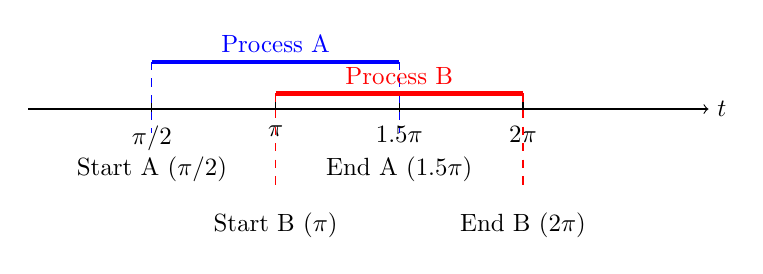
\begin{tikzpicture}[scale=1, every node/.style={scale=0.9}] % Adjust scale if needed
                \pgfmathsetmacro{\pival}{3.14159}
                \pgfmathsetmacro{\halfpi}{\pival/2}
                \pgfmathsetmacro{\oneandhalfpi}{1.5*\pival}
                \pgfmathsetmacro{\twoandhalfpi}{2.5*\pival} % Retain for x-axis range if desired, though B ends earlier now

                % Define the x-axis
                \draw[->] (0,0) -- (2.75*\pival,0) node[right] {$t$}; % Adjusted x-axis to better fit new range

                % X-axis ticks and labels
                \foreach \x/\labeltext in {\halfpi/{$\pi/2$}, \pival/{$\pi$}, \oneandhalfpi/{$1.5\pi$}, 2*\pival/{$2\pi$}} { % Removed 2.5pi tick, can be added back if needed
                \draw (\x,3pt) -- (\x,-3pt) node[below] {\labeltext};
                }

                % Process A (Blue)
                \draw[blue, ultra thick] (\halfpi, 0.6) -- (\oneandhalfpi, 0.6);
                \node[blue, above] at (\pival, 0.6) {Process A};
                \node[align=center, below] at (\halfpi, -0.5) {Start A ($\pi/2$)};
                \draw[blue, dashed] (\halfpi, 0.6) -- (\halfpi, -0.3);
                \node[align=center, below] at (\oneandhalfpi, -0.5) {End A ($1.5\pi$)};
                \draw[blue, dashed] (\oneandhalfpi, 0.6) -- (\oneandhalfpi, -0.3);

                % Process B (Red) - Overlapping A
                \draw[red, ultra thick] (\pival, 0.2) -- (2*\pival, 0.2); % Starts at pi, ends at 2*pi
                \node[red, above] at (\oneandhalfpi, 0.2) {Process B}; % Midpoint of B is 1.5*pi
                \node[align=center, below] at (\pival, -1.2) {Start B ($\pi$)};
                \draw[red, dashed] (\pival, 0.2) -- (\pival, -1.0);
                \node[align=center, below] at (2*\pival, -1.2) {End B ($2\pi$)};
                \draw[red, dashed] (2*\pival, 0.2) -- (2*\pival, -1.0);

            \end{tikzpicture}
            \caption{Timing diagram illustrating strategic sequencing of group finalizations, which can represent potential "nullifiable exit events." At such an event (e.g., "End A" or "End B"), a participant or group might convert achieved rank into governance power or a claim on the Rewards Treasury (as discussed in Section \ref{sec:utility_and_treasury}). Both illustrative groups (A and B) have the same characteristic election duration $T_{type}=\pi$. Group B initiates its process when Group A is halfway through its own, leading to a significant overlap. This demonstrates how competing efforts or coalitions might strategically time their periods of maximum potential influence or rank-to-governance conversion opportunities, potentially operating with phased dominance to maximize influence or manage resource claims over time. This overlap highlights the temporal dynamics of influence within the system.}
            \label{fig:processes}
        \end{figure}

        If many groups allocate their reasoning power in alliance, more complicated systems can be imagined. These can create local influence resonances, analyzable in frequency domain, to predict future behavior like illustrated in Fig. \ref{fig:processes-sinusoidal}.

        \begin{figure}[ht]
            \centering
            \begin{tikzpicture}
                % Define the x-axis
                \draw[->] (0,0) -- (10,0) node[right] {$T_{type,id1}=T_{type,id2}$};

                % Define the y-axis
                \draw[->] (0,-2) -- (0,2) node[above] {Collective Influence};

                % Define the first process (sine wave)
                \draw[domain=0:10,smooth,variable=\t,blue] plot ({\t},{sin(360*\t/10)});
                \node[blue] at (10,1) {Coalition 1};

                % Define the second process (sine wave shifted by half period)
                \draw[domain=0:10,smooth,variable=\t,red] plot ({\t},{sin(360*\t/10 + 180)});
                \node[red] at (10,-1) {Coalition 2};

                % Add labels for the half period shift
                \draw[dashed] (5,-2) -- (5,2);
                \node at (5,-2.5) {$\pi$};

                % Add labels for the full period
                \draw[dashed] (10,-2) -- (10,2);
                \node at (10,-2.5) {$2\pi$};

            \end{tikzpicture}
            \caption{Diagram showing two competing opinion groups over the same subject with the same characteristic duration $T_{type}$ but a $\pi$ phase difference. Sinusoidal waves illustrate their ability to strategically allocate their ranking on the time axis. In reality, groups (types) may have different $T_{type}$ values and could be more complex.
                \label{fig:processes-sinusoidal}}
        \end{figure}


        This dynamic interplay of strategically timed group activities and the potential for phased dominance by different coalitions, as illustrated abstractly in Fig. \ref{fig:processes} and Fig. \ref{fig:processes-sinusoidal}, is not merely a feature of competitive interaction but also an emergent sign of a functioning meritocracy. The ability for different competent groups to rise, exert influence (potentially converting rank to governance or treasury claims), and then make way for others, all based on sustained, validated effort and resource commitment, prevents entrenched monopolies of power. Such a system, where influence is fluid and tied to ongoing, demonstrated competence, can be seen as a prerequisite for building next-generation decentralized infrastructure. In this vision, critical user-facing services or endpoints might be managed and innovated upon by numerous independent, specialized groups (guilds or coalitions identified through ACIP). These groups, while autonomous and potentially in competitive phases for influence or resources, would nevertheless be incentivized to collaborate for the overall health and commonwealth of the ecosystem that sustains their recognition and rewards. This model of inter-group collaboration, underpinned by a meritocratic and dynamic allocation of influence, offers a pathway towards more resilient, adaptive, and equitably governed digital infrastructure.

        \subsection*{Utility of Participation Costs and the Rewards Treasury}\label{sec:utility_and_treasury}
        The primary economic innovation and long-term incentive of ACIP lies in the strategic use of participation costs, particularly the $X_{id,reward}$ component, to fund a communal \textbf{Rewards Treasury}. This treasury is not merely a passive pool of assets; its allocation and governance are intended to be managed by participants who have achieved and maintain significant rank, representing a second, higher-order layer of peer recognition and collective stewardship.

        It is crucial to recognize that the "participation costs," particularly the $X_{id,reward}$ component notionally funding the Rewards Treasury, need not always represent direct, liquid financial contributions. The protocol allows for flexibility where these commitments can be evidenced by verifiable, non-transferable proofs of engagement or contribution to a specific ecosystem. For example, facts of active subscriptions to a platform, cryptographically verifiable receipts for service usage, or even tokens issued as remuneration for gas spent on a blockchain could qualify as valid "entry tickets" or commitments for participating in ACIP groups within that platform's context. Similarly, an educational institution could issue such qualifying credits based on tuition fees paid or academic milestones achieved, allowing participation in competence groups relevant to its domain.

        In such scenarios, the Rewards Treasury itself might not primarily accumulate assets with direct, intrinsic market value in the traditional sense; instead, it could represent a pool of these "receipt-value" attestations or rights. While this form of treasury still underpins the seriousness of participation and the value of achieved rank within that specific ecosystem, the direct financial incentivization might be different. However, this does not preclude the possibility of implementing an additional, parallel bounty system. Such a system could be funded through other means (e.g., a portion of any actual monetary fees, external grants, or contributions from ecosystem stakeholders) to provide more tangible, market-valued rewards for exceptional performance or for achieving universally recognized high ranks, complementing the ecosystem-specific value represented in the primary Rewards Treasury.



        While a minor fraction of $X_{id,reward}$ from an individual group competition might be allocated as an immediate incentive to the direct winner (kept below levels that would make single-group Sybil attacks profitable, as per Eq. \ref{eq:sybil_cost_one_group_expected}), the substantial portion of these collected reward components across all groups continuously funds the main Rewards Treasury.

        The core utilities and game-theoretic implications are:
        \begin{itemize}
            \item \textbf{The Rewards Treasury as a Central Incentive:} This collectively managed treasury can grow to a significant Total Value Locked (TVL). Access to, and governance over, this treasury becomes a primary driver for long-term, legitimate participation and rank progression. It represents the shared success and accumulated value recognized by the community.

            \item \textbf{Governance by High-Rank Coalitions:} Established high-rank participants (forming an \textit{incumbent ruling coalition} or a recognized body of peers) are envisioned to govern the rules for the Treasury's allocation. This includes defining mechanisms for distributing rewards, funding proposals, or other collectively beneficial initiatives. This governance itself is a form of advanced peer recognition.

            \item \textbf{Rank Conversion (Legitimate Value Realization):} To provide a tangible return for sustained competence and investment, high-rank participants may be offered a mechanism to voluntarily "nullify" or convert their achieved rank into a claim on a portion of the Rewards Treasury, or into specific governance rights over it. The "exchange rate" or conditions for this conversion must be carefully designed. Crucially, the effective cost to the individual for this legitimate "cash-out" (in terms of rank surrendered) should be evaluated against the cost an attacker would face to illicitly achieve that same rank and attempt a similar extraction ($C_{TotalSybilToRankR}$ from Eq. \ref{eq:total_sybil_cost_to_rank_R}). The aim is to make legitimate realization of value through sustained participation more favorable than Sybil-based extraction.

            \item \textbf{Treasury as Staking Collateral for Guild-Endorsed Competence:} A significant utility of the Rewards Treasury is its potential to serve as a staking asset for \textit{Competence Guilds}—organizations formed by high-ranking participants often focused on specific domains or dimensions of competence (e.g., a "Technical Guild" or a "Strategy Guild"). These guilds, through their established collective competence (represented by their members' aggregated competence vectors) and governance, could be allocated or earn the right to manage portions of the Treasury. They can then use these assets to "bake" or stake against the ACIP competence vectors (or specific dimensional components thereof) of individuals they rigorously vet and endorse. This act of a guild staking its treasury portion transforms a member's competence attestation into a directly collateralized \textbf{Guild-Backed Proof of Competence} for the endorsed dimension(s) or profile. This significantly enhances the competence signal's power and trustworthiness, as it is now vouched for by the tangible value and collective reputation of the guild within its specific domain. This creates strong incentives for guilds to maintain high standards in their endorsement processes, as their staked treasury portion could be at risk (e.g., slashed or devalued) if their endorsed members act incompetently or maliciously within the endorsed dimensions, depending on the specific guild and protocol rules.

            \item \textbf{Sunk Costs for Protocol Operation:} The $X_{id,data}$ and $X_{id,comp}$ components of participation costs are directed towards essential protocol operations. This includes ensuring data retention for group interactions and competition history (e.g., leveraging systems like CVPP \cite{cvpp} or Swarm \cite{swarm}) and covering ongoing computational and network transaction fees. These are non-recoverable operational expenses for all participants, including attackers, ensuring the protocol's sustainability.

            \item \textbf{Enhanced Economic Incentives:} The existence of a substantial, collectively governed Rewards Treasury—now also serving as a potential source of collateral for guild-backed competence—significantly amplifies the economic incentive beyond intrinsic interest in discussion topics. It transforms ACIP rank into a potent reputation with tangible economic backing and governance potential, making legitimate, long-term participation highly attractive.

            \item \textbf{Defense of the Treasury:} As discussed in Section \ref{sec:time-constraint}, the governance structure of the Rewards Treasury by established high-rank peers, combined with the time-delay inherent in achieving high rank, provides a mechanism to defend the treasury against hostile takeovers by rapidly ascending Sybil attackers. Non-acceptance of a new, suspicious high-rank entity by the incumbent peerage can manifest as safeguarding the treasury and its capacity to back legitimate competence.

        \end{itemize}
        The precise mechanisms for Treasury governance, rank conversion, and guild-staking operations are critical design elements that would be detailed in specific implementation proposals and are subject to the evolution of the protocol through its own potential governance processes.

        \subsection{Synergies with Data-Driven Systems and Machine Learning}
        \label{sec:ml_synergies}

        Beyond its direct applications in governance and reputation, ACIP, particularly when integrated with content-generation or problem-solving protocols like CVPP \cite{cvpp}, offers a powerful framework for creating and validating high-quality, domain-specific datasets suitable for Machine Learning (ML) applications. The multi-dimensional competence structure further enhances this capability.

        \begin{itemize}
            \item \textbf{Generation of Distilled, Ranked, and Ordered Datasets:} The core ACIP process, where participants engage in competitive tasks within dimension-specific groups, naturally produces a stream of data (e.g., code, analyses, designs, arguments, curated information). This data is:
                  \begin{itemize}[label=\textbullet, leftmargin=*]
                      \item \textit{Distilled and Categorized:} Tied to the specific competence dimension the group is focused on, providing clear thematic categorization.
                      \item \textit{Ranked and Validated:} The election process and the resulting ranks of contributors act as an inherent quality filter and validation mechanism. Contributions from higher-ranked individuals or winning submissions can be considered of higher quality or greater relevance.
                      \item \textit{Ordered:} The progression of ranks provides a natural ordering of expertise, which can be valuable for curriculum learning or for weighting data contributions in ML models.
                  \end{itemize}
                  Such datasets are directly usable for training and fine-tuning ML models in specialized areas, as the competence dimensions themselves serve as robust labels or categories. {{The focus on peer-validated, high-effort contributions can also serve as a potential mitigation against issues like \textit{model collapse} or \textit{autophagy}, where models trained predominantly on their own or other AI-generated output can degrade in quality and diversity \cite{dohmatob2024strongmodelcollapse}.}}

            \item \textbf{A Financial and Reputational Model for Agent Evaluation:} ACIP provides a transparent and economically grounded model for evaluating the competence of any participating agent, be it human or an AI model itself participating in ACIP challenges. The costs incurred ($X_{id}$) and the rank achieved ($\vec{P_r}$) offer quantifiable metrics of commitment and peer-validated skill. This can be used to:
                  \begin{itemize}[label=\textbullet, leftmargin=*]
                      \item Identify and reward high-quality data labelers or contributors.
                      \item Evaluate the performance of AI models trained on ACIP-generated data by having them participate in competence challenges.
                      \item Create incentive structures for continuous improvement of both human and AI agents within specific competence domains.
                  \end{itemize}

            \item \textbf{Comparison to Existing Data Mechanisms:}
                  \begin{itemize}[label=\textbullet, leftmargin=*]
                      \item \textit{Crowdsourcing Platforms (e.g., Mechanical Turk):} Often struggle with ensuring deep domain expertise for complex tasks and maintaining consistent quality. Incentives may not align with the production of high-fidelity, nuanced data. ACIP, by contrast, is designed to select for and reward domain-specific competence, leading to potentially higher-quality data from verifiably skilled participants.
                      \item \textit{Expert Labeling/Curation:} While producing high-quality data, this approach is typically expensive, slow to scale, and centralized. ACIP offers a decentralized and potentially more scalable model for identifying and leveraging domain experts (high-rank participants and guilds) for data generation, validation, and curation tasks.
                      \item \textit{Unstructured Web Data:} Vast but often noisy, unverified, and lacking clear signals of quality or contextual relevance. {{Training on such data without robust filtering can contribute to model degradation phenomena like model collapse \cite{dohmatob2024strongmodelcollapse}.}} ACIP-generated datasets are inherently structured around competence dimensions, peer-validated, and context-rich.
                  \end{itemize}
        \end{itemize}
        The synergy between ACIP's competence validation and the need for high-quality, specialized data for advanced AI systems presents a significant avenue for future development and application, creating a positive feedback loop where competence in generating valuable data is itself a dimension that can be ranked and rewarded within the ACIP framework.

        \section{Conclusion}
        This paper introduces a novel protocol for establishing a dynamic ranking ladder system in trustless environments. Our protocol enables autonomous identification while mitigating Sybil attacks by leveraging game-theoretic principles and dynamic systems theory. The time-based and cost-based mechanisms ensure high ranks require genuine effort and skill, and opposite opinions can co-exist. {{The potential for multi-dimensional competence representation, governed Rewards Treasuries that can back attested rank tokens via Competence Guilds, and the generation of high-quality, validated datasets for Machine Learning further extend ACIP's utility beyond simple ranking.}}

        This protocol offers a foundation for building more robust and equitable decentralized governance systems. It improves blockchain consensus mechanisms, enhances DAO decision-making, and fosters healthier online communities.

        Further work is needed to analyze the protocol's behavior and effectiveness using dynamic system theory and explore its integration with existing decentralized platforms. {{Key areas for future research include the detailed modeling of multi-dimensional competence dynamics, the economic and game-theoretic implications of guild-based rank-backing, and the practical implementation of ACIP as an engine for generating competence-validated datasets for AI development.}}

        The importance of transparency and participant agency in choosing groups and forming alliances is highlighted as a key component of collusion resistance, moving away from reliance on a separate, undefined clustering system.

        Due to the principal components of time and cost, the protocol can support a large number of groups, ensuring maximized scalability and adaptability to diverse needs.

        A roadmap for integrating this protocol into existing decentralized platforms will be provided in follow-up works.

        The utility of locked funds is multifaceted: it is used to retain data about competitions, optionally serves as a funding source for protocol operations, and most importantly, functions as TVL locked within the representation of competence. This TVL allows the Proof of Competence to be quantified in both financial and temporal terms.

        In comparison to existing solutions, our protocol distinguishes itself by not enforcing specific KYC requirements and by using the social graph as an auxiliary tool for collusion clustering rather than a central component. This makes it a valuable and complementary addition to systems that rely on stricter identity verification methods.

        Furthermore, unlike purely reputation-based systems that can be slow to adapt and vulnerable to initial bias, ACIP's dynamic ranking ladder offers a more responsive and continuously updated measure of competence. Compared to systems relying solely on subjective peer review, ACIP introduces objective cost and time commitments, making competence harder to fake and easier to verify. When contrasted with established pairwise comparison models like the Bradley-Terry model, which infers probabilities of one item or participant being preferred over another, or rating systems such as Elo, commonly used in competitive games to estimate relative skill levels, ACIP presents several distinctions. While Bradley-Terry and Elo are effective for deriving relative rankings from dyadic interactions or zero-sum outcomes, ACIP is designed for a broader context. It explicitly incorporates multi-dimensional competence vectors rather than a single skill score, integrates economic and temporal commitments ($X_{id}$, $T_{id}$) as foundational elements for rank progression and Sybil resistance, and focuses on a richer group-based competitive interaction (the "election" process) which can be more complex than simple pairwise outcomes. Moreover, ACIP aims to build a framework for collective reward governance through its Rewards Treasury and guild structures, an aspect typically outside the scope of traditional rating systems. While the internal mechanics of ACIP's group competitions might draw inspiration from or even incorporate elements of such models for specific types of challenges, its overarching architecture for autonomous competence identification and its economic underpinnings are distinct. ACIP can be seen as complementary to existing decentralized identity and reputation solutions, providing a robust and dynamic competence layer that can enhance their effectiveness.


    \clearpage

    \bibliographystyle{ieeetr}
    \bibliography{../references.bib}

    \clearpage\end{CJK}
\end{document}
